\documentclass[aspectratio=169]{beamer}

\mode<presentation>
{
  \usetheme{default}
  \usecolortheme{default}
  \usefonttheme{default}
  \setbeamertemplate{navigation symbols}{}
  \setbeamertemplate{caption}[numbered]
  \setbeamertemplate{footline}[frame number]  % or "page number"
  \setbeamercolor{frametitle}{fg=white}
  \setbeamercolor{footline}{fg=black}
} 

\usepackage[english]{babel}
\usepackage[utf8x]{inputenc}
\usepackage{tikz}
\usepackage{courier}
\usepackage{array}
\usepackage{bold-extra}
\usepackage{minted}
\usepackage[thicklines]{cancel}

\xdefinecolor{dianablue}{rgb}{0.18,0.24,0.31}
\xdefinecolor{darkblue}{rgb}{0.1,0.1,0.7}
\xdefinecolor{darkgreen}{rgb}{0,0.5,0}
\xdefinecolor{darkgrey}{rgb}{0.35,0.35,0.35}
\xdefinecolor{darkorange}{rgb}{0.8,0.5,0}
\xdefinecolor{darkred}{rgb}{0.7,0,0}
\definecolor{darkgreen}{rgb}{0,0.6,0}
\definecolor{mauve}{rgb}{0.58,0,0.82}

\title[2017-10-25-aps-nuclear]{Bridging the Particle Physics and Big Data Worlds}
\author{Jim Pivarski}
\institute{Princeton University -- DIANA-HEP}
\date{October 25, 2017}

\begin{document}

\logo{\pgfputat{\pgfxy(0.11, 7.4)}{\pgfbox[right,base]{\tikz{\filldraw[fill=dianablue, draw=none] (0 cm, 0 cm) rectangle (50 cm, 1 cm);}\mbox{\hspace{-8 cm}
\includegraphics[height=1 cm]{princeton-logo-long.png}
\includegraphics[height=1 cm]{diana-hep-logo-long.png}}}}}

\begin{frame}
  \titlepage
\end{frame}

\logo{\pgfputat{\pgfxy(0.11, 7.4)}{\pgfbox[right,base]{\tikz{\filldraw[fill=dianablue, draw=none] (0 cm, 0 cm) rectangle (50 cm, 1 cm);}\mbox{\hspace{-8 cm}
\includegraphics[height=1 cm]{princeton-logo.png}
\includegraphics[height=1 cm]{diana-hep-logo.png}}}}}

% Uncomment these lines for an automatically generated outline.
%\begin{frame}{Outline}
%  \tableofcontents
%\end{frame}

%%%%%%%%%%%%%%%%%%%%%%%%%%%%%%%%%%%%%%%%%%%%%%%%%%%%%%%

%%%% START

\begin{frame}{Particle physics: the original Big Data}
\vspace{0.5 cm}

\large For decades, our computing needs were unique:

\vspace{0.1 cm}
\begin{itemize}
\item large datasets \hfill \begin{minipage}{0.7\linewidth}(too big for one computer: a moving definition!),\end{minipage}
\item complex structure \hfill \begin{minipage}{0.7\linewidth}(nested data, web of relationships within each event),\end{minipage}
\item has to be reduced \hfill \begin{minipage}{0.7\linewidth}(aggregated, by histogramming, usually)\end{minipage}
\item to be modeled \hfill \begin{minipage}{0.7\linewidth}(fitting to extract physics results).\end{minipage}
\end{itemize}

\vspace{0.5 cm}
\uncover<2->{\textcolor{darkblue}{\large Today these criteria apply equally, or more so, to ``web scale data.''}}
\end{frame}

\begin{frame}{{200~PB is a lot of data}\only<2>{, but for Amazon, it's two truckloads}}
\vspace{0.35 cm}
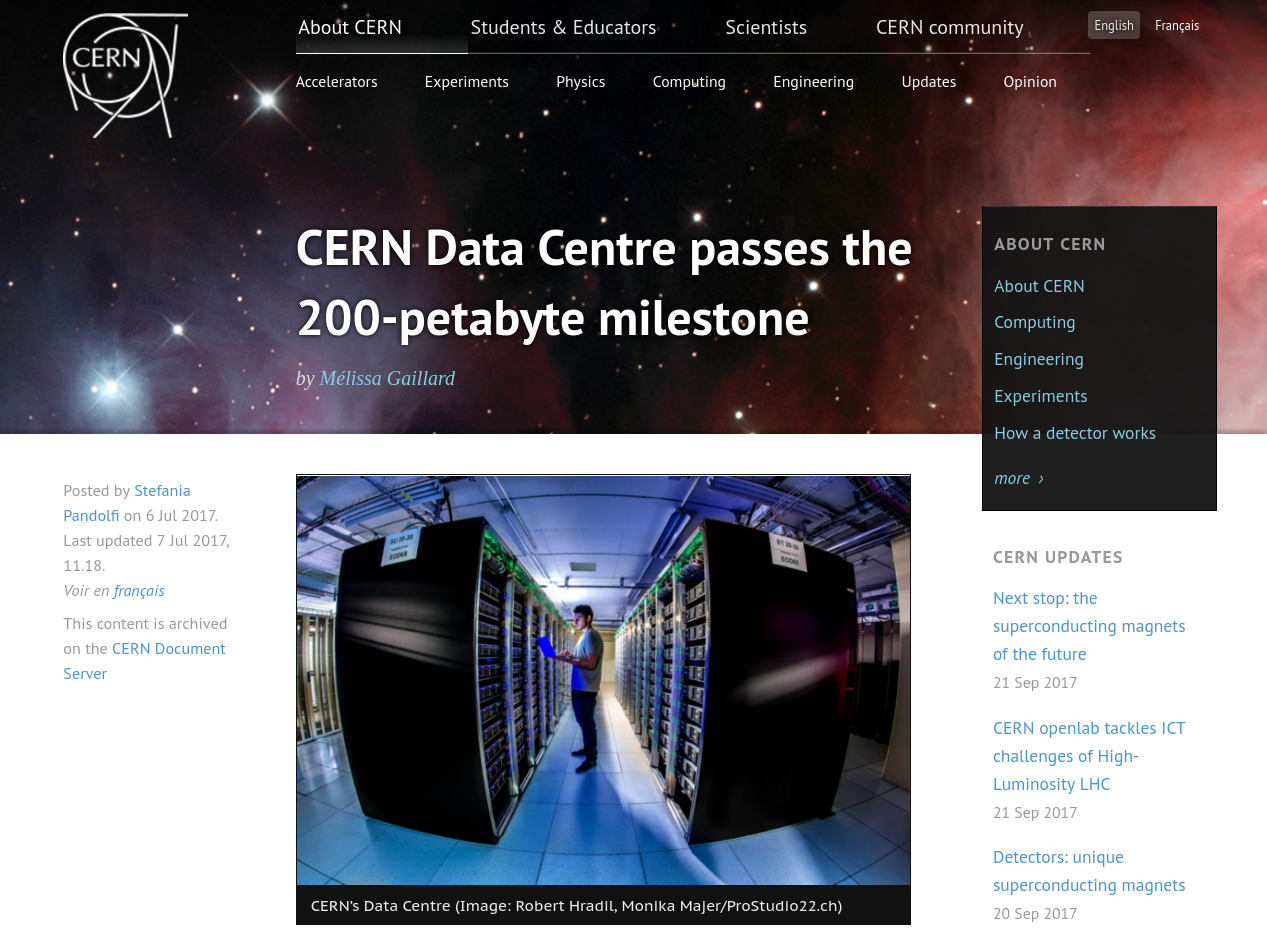
\includegraphics[width=0.73\linewidth]{cern-200pb.png}

\vspace{-4.8 cm}
\uncover<2->{\mbox{ } \hfill 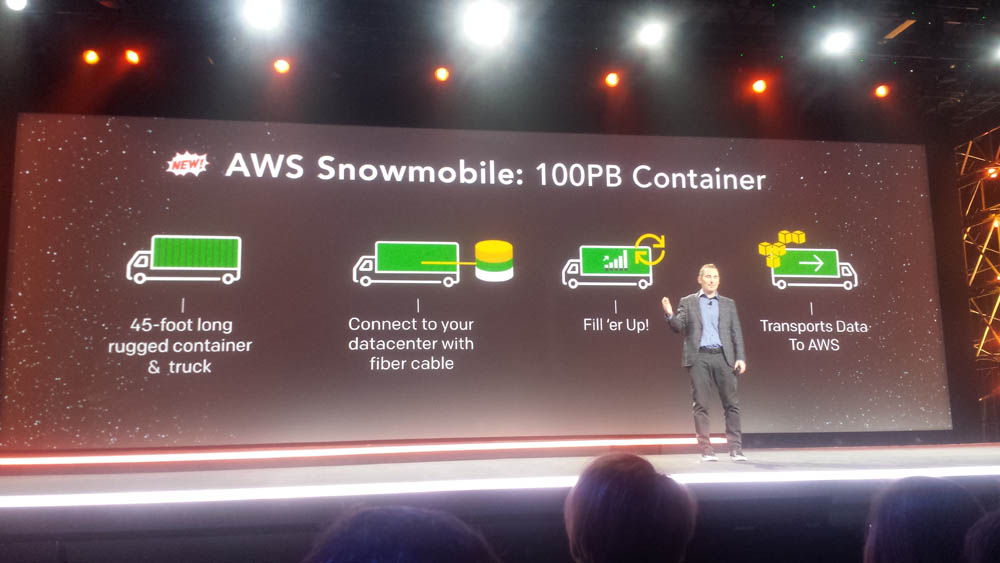
\includegraphics[width=0.7\linewidth]{aws-snowmobile.jpg}\hspace{-1 cm}}
\end{frame}

\begin{frame}{Also a much larger community}
\vspace{0.35 cm}
\textcolor{darkblue}{Rate of web searches for ``ROOT TTree'' vs.\ ``Spark DataFrame'' (Google Trends):}

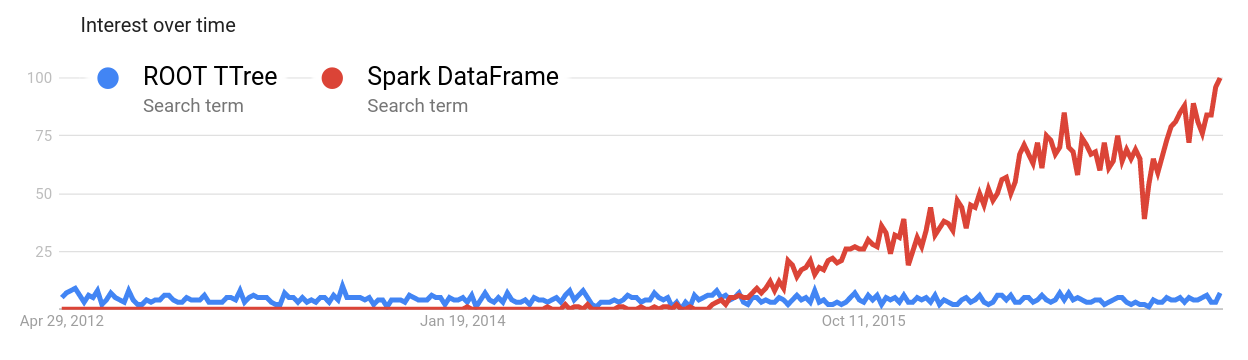
\includegraphics[width=\linewidth]{root-spark-google-trends.png}

\vfill
\begin{uncoverenv}<2->
\textcolor{darkblue}{Similarly for question-and-answer sites:}
\begin{itemize}
\item RootTalk: 14,399 threads in 1997--2012 (15 years)
\item StackOverflow questions tagged {\tt \small \#spark}: 26,155 in the 3.3 years the tag has existed. (Not counting CrossValidated, Spark Developer and User mailing lists\ldots)
\end{itemize}
\end{uncoverenv}

\vfill
\uncover<3>{\textcolor{darkorange}{\bf More users to talk to; more developers adding features/fixing bugs.}}
\end{frame}

\begin{frame}{Particle physics is a special case}
\vspace{-0.5 cm}
\begin{columns}[t]
\column{0.5\linewidth}
\begin{center}
\underline{\Large Particle physics}
\end{center}

\begin{itemize}
\item Events (modulo cosmics vetos or time-dependent calibrations) may be processed in isolation; embarrassingly parallel.

\item<2-> Once collected, physics datasets are immutable (with revisions).

\item<3-> Often fitting a model with a small number of parameters.

\end{itemize}

\column{0.5\linewidth}
\begin{center}
\underline{\Large Big Data}
\end{center}

\begin{itemize}
\item All-to-all problems are common, such as matching a customer's purchases with all other purchases to make a recommendation.

\item<2-> Transactions accumulate in the database during analysis.

\item<3-> Modeling human behavior, more interested in predictions than description, so models may have thousands of free parameters.

\end{itemize}

\end{columns}
\end{frame}

\begin{frame}{Our software is largely isolated from these developments}
\vspace{0.17 cm}
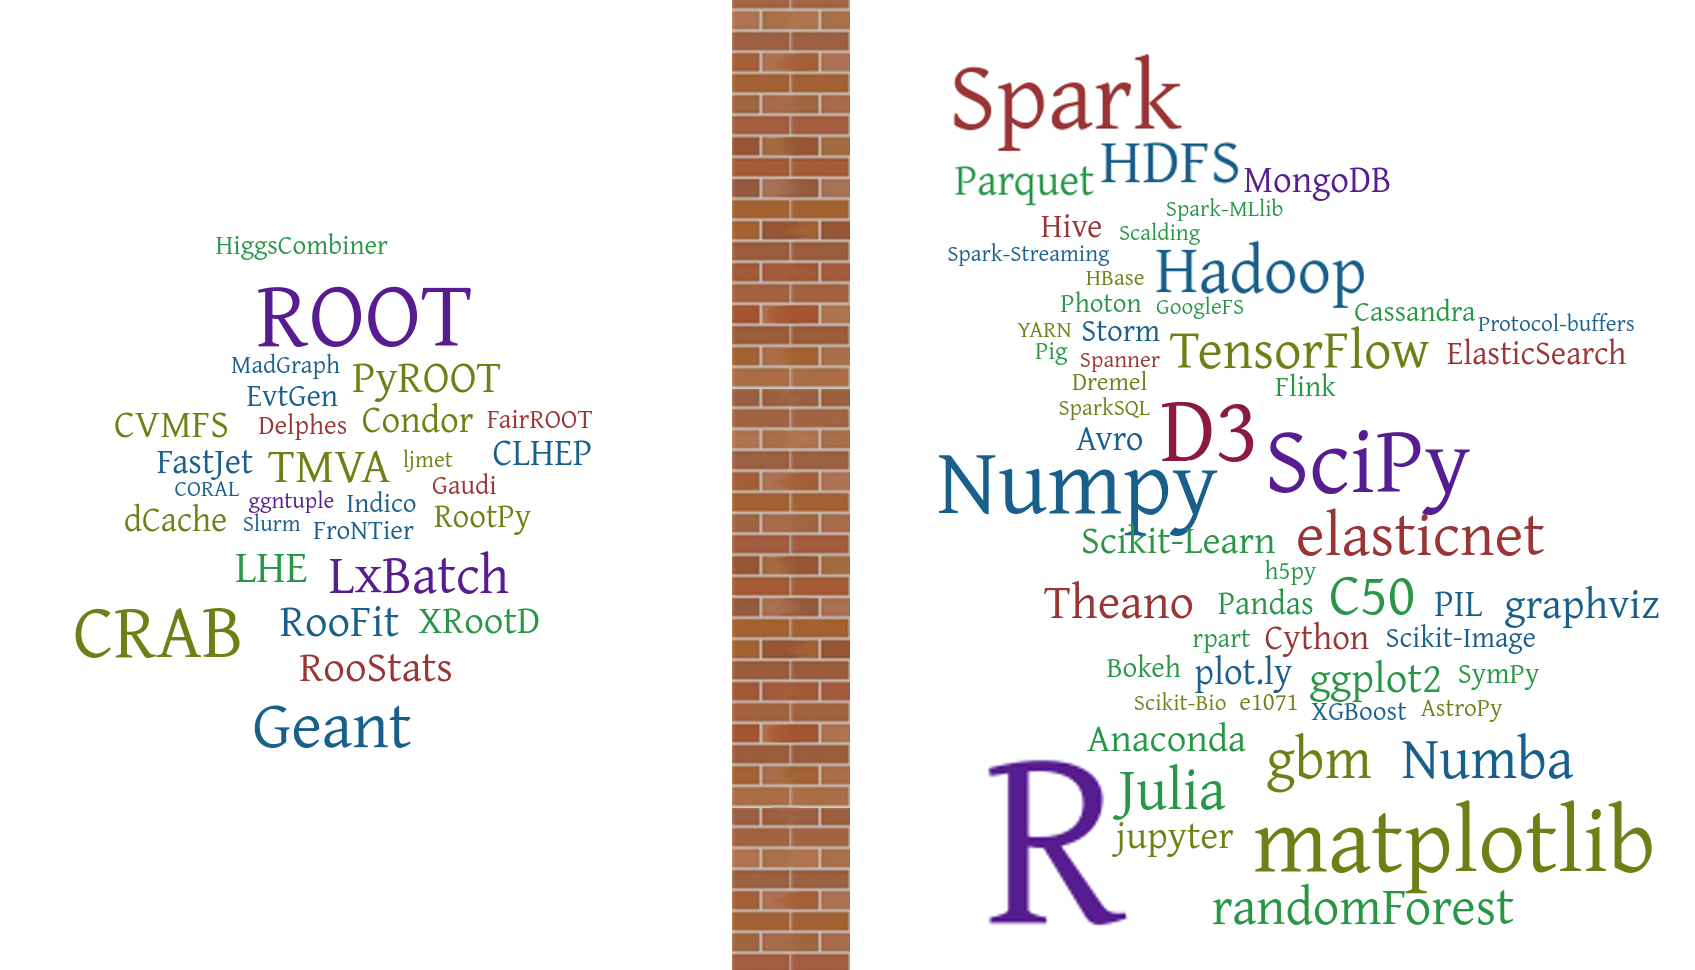
\includegraphics[width=\linewidth]{separation-2.png}
\end{frame}

\begin{frame}{Who am I? Why am I giving this talk?}
\vspace{0.5 cm}
\begin{columns}[t]
\column{0.4\linewidth}
\begin{columns}
\column{0.4\linewidth}
Jim Pivarski
\column{0.25\linewidth}
\hspace{-1.3 cm}
\includegraphics[width=\linewidth]{jim_pivarski.png}
\end{columns}

\begin{itemize}
\item 5 years CLEO (9 GeV $e^+e^-$)
\item 5 years CMS (7 TeV $pp$)
\item \only<1>{5 years Open Data Group}\only<2->{\mbox{\textcolor{darkblue}{5 years Open Data Group \hspace{0.9 cm}$\longrightarrow$\hspace{-3 cm}}}}
\item 2 years Project DIANA-HEP
\end{itemize}

\column{0.4\linewidth}
\uncover<2->{\textcolor{darkblue}{
hyperspectral imagery \\
automobile traffic \\
network security \\
Twitter sentiment \\
Google n-grams \\
DNA sequence analysis \\
credit card fraud detection
}}

\uncover<2->{\Large\textcolor{darkblue}{ and ``Big Data'' tools}}
\end{columns}

\vspace{0.5 cm}
\begin{center}
\uncover<3>{\textcolor{violet}{\bf My goal within DIANA-HEP is to make it easier for physicists to use Big Data tools in their analyses, particularly for interactive, exploratory analysis.}}
\end{center}
\end{frame}

\begin{frame}{}
\vspace{-0.22 cm}
\begin{center}
\only<1>{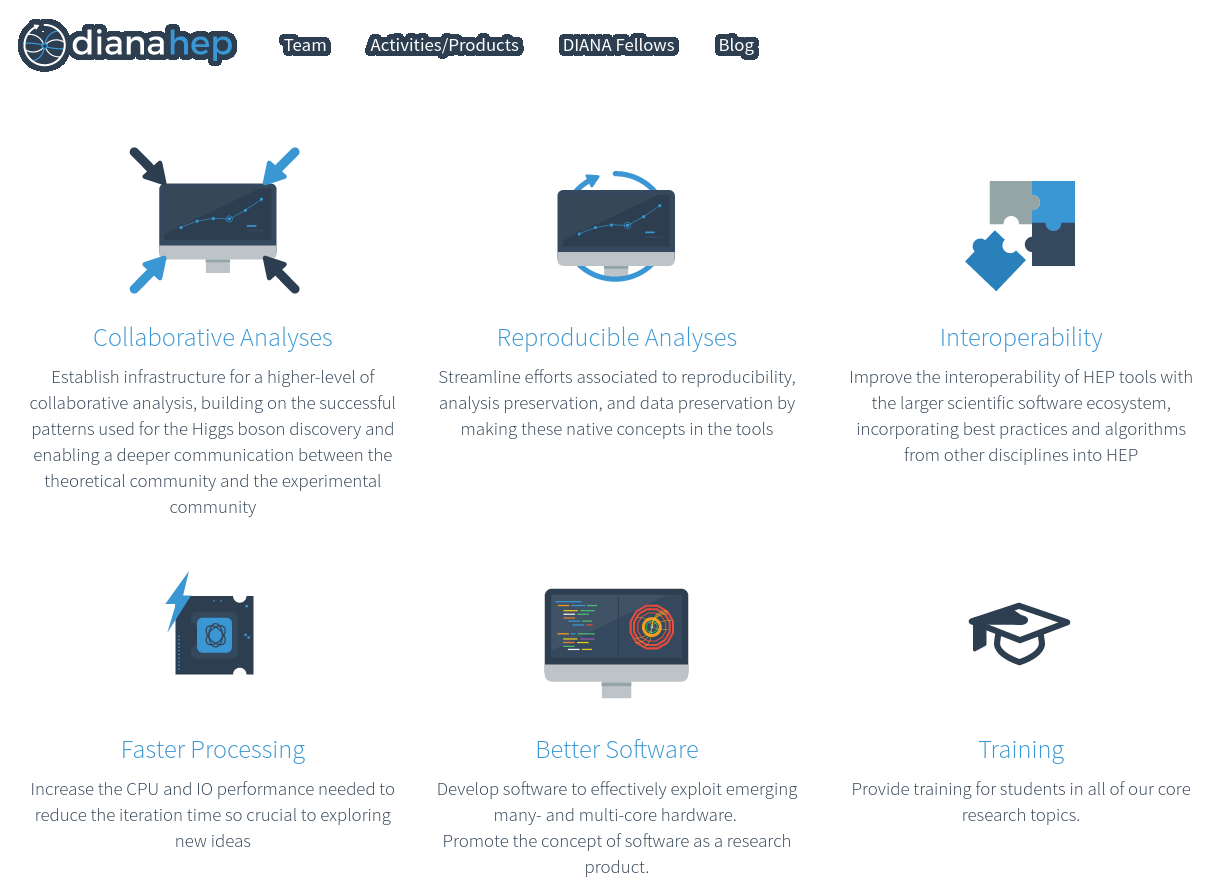
\includegraphics[width=0.88\linewidth]{diana-hep.png}}
\only<2>{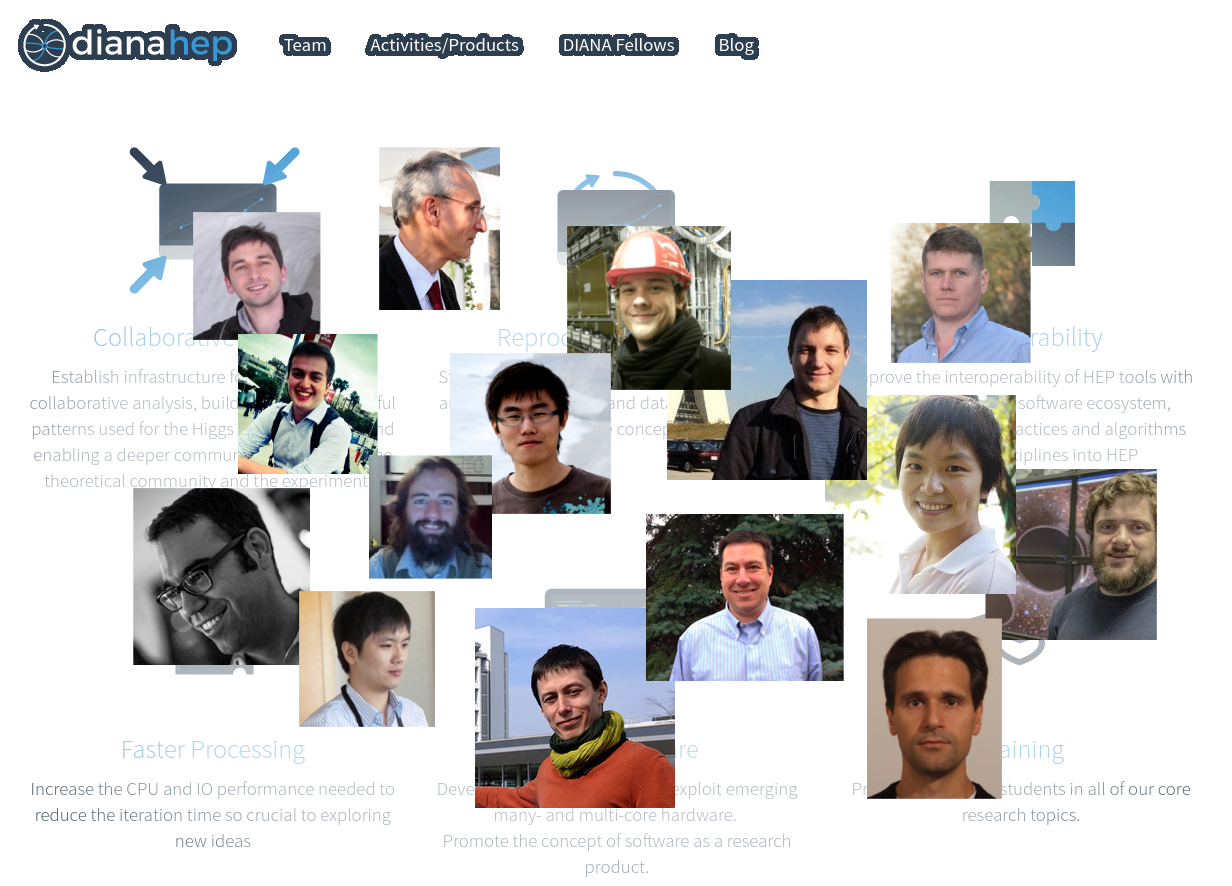
\includegraphics[width=0.88\linewidth]{diana-hep2.png}}
\end{center}
\end{frame}

\begin{frame}{What to do with physics software: three cases}
\vspace{0.25 cm}
\begin{columns}[t]
\column{0.33\linewidth}
\textcolor{darkblue}{\underline{Case I:}} Physics software that serves {\it the same function} as software in the Big Data community.

\begin{uncoverenv}<2->
\begin{center}

\includegraphics[height=1.5 cm]{stamp_replace.png}
\end{center}

Big Data community has better resources for
\begin{itemize}
\item maintaining code
\item catching bugs
\item revising bad designs.
\end{itemize}
\end{uncoverenv}

\column{0.33\linewidth}
\textcolor{darkblue}{\underline{Case II:}} Domain-specific software for our analyses. Example: ``HiggsCombiner.'' \mbox{\hspace{1 cm}}

\begin{uncoverenv}<3->
\begin{center}

\includegraphics[height=1.5 cm]{stamp_keep.png}
\end{center}

Obviously. This really is a unique problem.
\end{uncoverenv}

\column{0.33\linewidth}
\textcolor{darkblue}{\underline{Case III:}} Physics software or concepts that would benefit the Big Data community. \\ \mbox{ }

\begin{uncoverenv}<4->
\begin{center}

\includegraphics[height=1.5 cm]{stamp_promulgate.png}
\end{center}

Cultural exchange goes in both directions.
\end{uncoverenv}
\end{columns}
\end{frame}

\begin{frame}{}
\vspace{0.5 cm}
\begin{center}
\begin{minipage}{0.8\linewidth}
\begin{center}
\Large All three cases in a single story: porting an analysis from ROOT to Spark.
\end{center}
\end{minipage}
\end{center}
\end{frame}

\begin{frame}{CMS Big Data Project}
\vspace{1 cm}
\begin{columns}
\column{0.4\linewidth}
\begin{itemize}
\item Oliver Gutsche, Matteo Cremonesi, Cristina Su\'arez (Fermilab) wanted to try their CMS dark matter search on Spark.
\item My first DIANA-HEP project: I joined to plow through technical issues before the analysts hit them.
\end{itemize}

\column{0.6\linewidth}
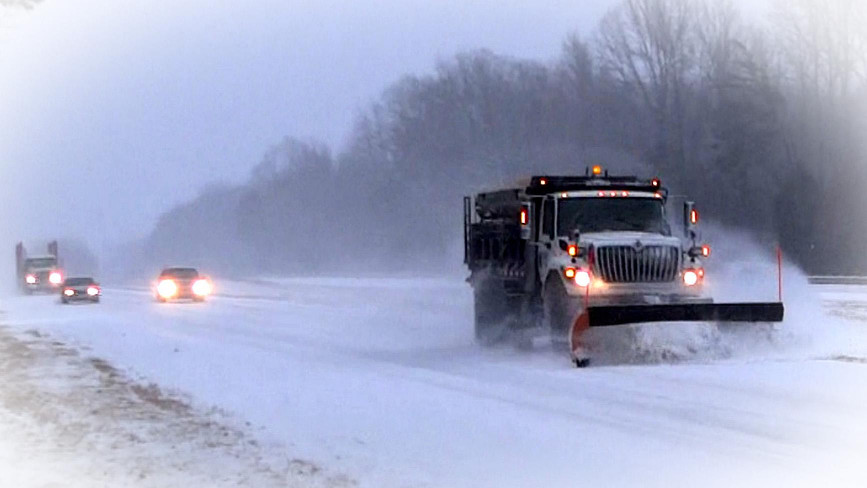
\includegraphics[width=\linewidth]{snowplow.jpg}
\end{columns}

\vspace{0.25 cm}
\begin{center}
\textcolor{blue}{\underline{\url{https://cms-big-data.github.io/}}}
\end{center}
\end{frame}

\begin{frame}{How to get the data into Spark (which runs in Java)}
\vspace{0.5 cm}
\small

\underline{\large \bf A year of trial-and-error in one slide}
\begin{center}
\begin{minipage}{0.8\linewidth}
\begin{enumerate}
\item \textcolor{darkblue}{Java Native Interface (JNI)} \\ No! This ought to be the right solution, but Java \\ and ROOT are both large, complex applications \\ with their own memory management: couldn't keep \\ them from interfering (segmentation faults).

\vspace{-2.2 cm}
\hfill 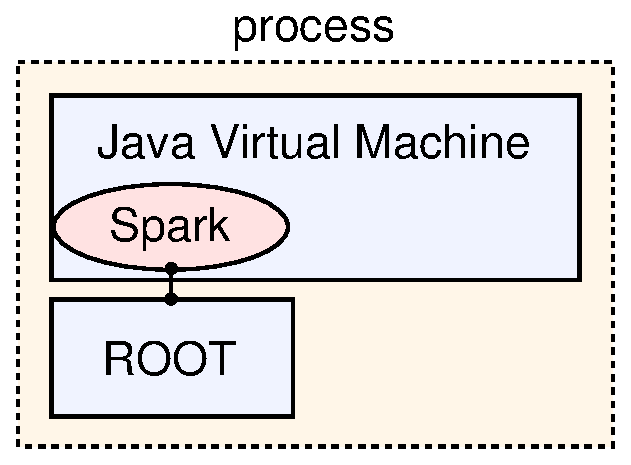
\includegraphics[height=1.65 cm]{root-spark.pdf}

\vspace{0.5 cm}
\item \textcolor{darkblue}{\normalsize Python as glue: PyROOT and PySpark in the same process}

\hfill 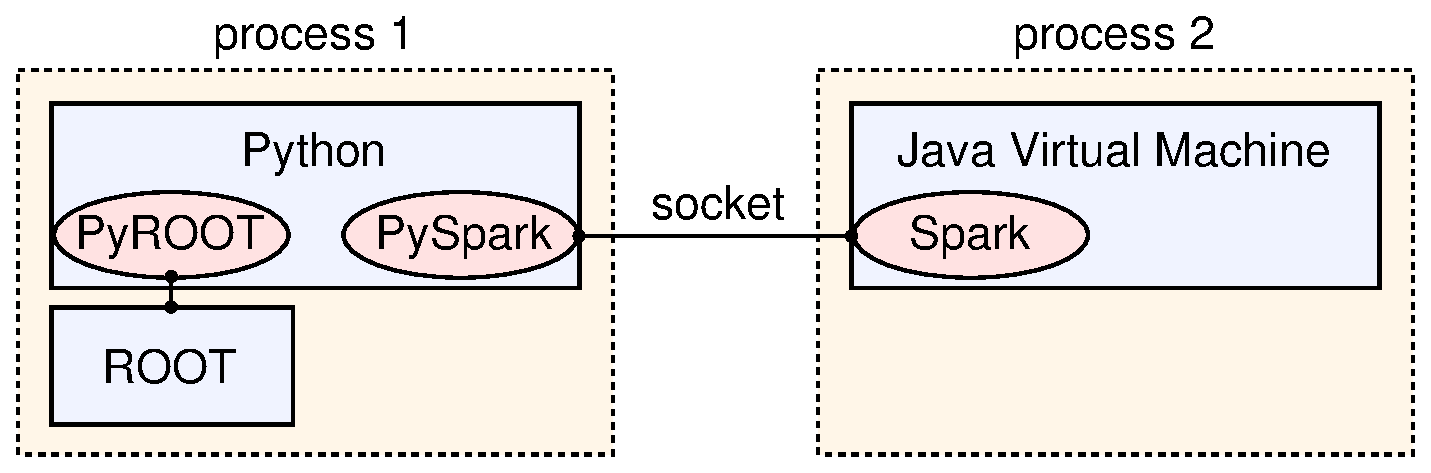
\includegraphics[height=1.65 cm]{pyroot-pyspark.pdf}

\vspace{-1.8 cm}
PySpark is a low-performance \\ solution: all data must be passed \\ over a text-based socket and \\ interpreted by Python.

\item \textcolor{darkblue}{\normalsize Convert to a Spark-friendly format, like Apache Avro}

We used this for most of the year. Efficient after conversion, but conversion step is awkward. Avro's C library is difficult to deploy.
\end{enumerate}
\end{minipage}
\end{center}

\begin{uncoverenv}<2->
\vspace{-5.2 cm}
\begin{center}
\fcolorbox{violet}{white}{\begin{minipage}{0.95\linewidth}
\vspace{0.5 cm}
\begin{center}
\begin{minipage}{0.95\linewidth}
\centering \large \textcolor{violet}{\bf This problem is incidental, not essential. Industry-standard formats like Avro and Parquet can store complex physics events; we just happen to have a lot of data in ROOT files.}
\end{minipage}
\end{center}
\vspace{0.1 cm}
\end{minipage}}
\end{center}
\vspace{5 cm}
\end{uncoverenv}
\end{frame}

\begin{frame}{This was a missed opportunity for exporting physics solutions!}
\vspace{0.5 cm}
\large \textcolor{violet}{\bf ROOT was storing nested data structures in a columnar format (for faster access) over a decade before it was reinvented at Google.}

\vspace{-0.3 cm}
\begin{center}
\begin{minipage}{0.8\linewidth}
\vspace{0.5 cm}
\small Sergey Melnik, Andrey Gubarev, Jing Jing Long, Geoffrey Romer, Shiva Shivakumar, Matt Tolton, Theo Vassilakis. \textcolor{darkblue}{\normalsize {\it Dremel: Interactive Analysis of Web-Scale Datasets} (2010).}

\vspace{0.25 cm}
\fbox{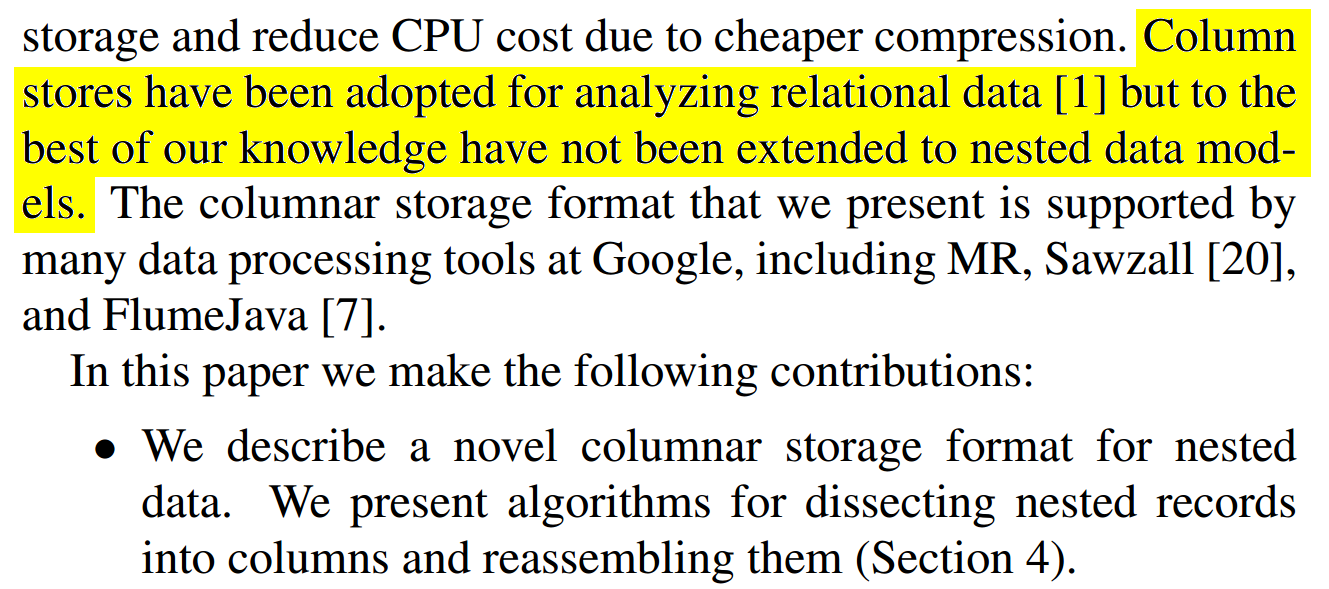
\includegraphics[width=\linewidth]{dremel-paper.png}}
\end{minipage}
\end{center}
\end{frame}

\begin{frame}{Easiest solution: reimplement ROOT I/O in Java\only<2->{, JS}\only<3->{, Go}\only<4->{, Python}}
\vspace{0.25 cm}
\begin{columns}
\column{1.1\linewidth}

\renewcommand{\arraystretch}{2.5}
\begin{tabular}{p{2 cm} c p{4.7 cm} p{5.25 cm}}
\centering \textcolor{red}{root4j/ spark-root} & \textcolor{red}{Java/Scala} & \textcolor{red}{For Spark and other Big Data projects that run on Java.} & \textcolor{red}{Started by Tony Johnson in 2001, updated by Viktor Khristenko.} \\
\centering \only<2->{\textcolor{darkgreen}{JsRoot}} & \only<2->{\textcolor{darkgreen}{Javascript}} & \only<1>{\mbox{\hspace{4 cm}} \mbox{\hspace{4 cm}}}\only<2->{\textcolor{darkgreen}{For interacting with ROOT in web browsers or standalone.}} & \only<2->{\textcolor{darkgreen}{Sergey Linev}} \\
\centering \only<3->{\textcolor{mauve}{rootio}} & \only<3->{\textcolor{mauve}{Go}} & \only<3->{\textcolor{mauve}{go-hep ecosystem in Go.}} & \only<3->{\textcolor{mauve}{Sebastien Binet}} \\
\centering \only<4->{\textcolor{blue}{uproot}} & \only<4->{\textcolor{blue}{Python}} & \only<1-3>{\mbox{\hspace{4 cm}} \mbox{\hspace{4 cm}} \mbox{\hspace{4 cm}}}\only<4->{\textcolor{blue}{For quickly getting ROOT data into Numpy and Pandas for machine learning.}}\vspace{-0.25 cm} & \only<4->{\textcolor{blue}{Jim Pivarski (me)}} \\
 & \only<5->{\textcolor{darkorange}{\bf Rust?}} & & \\
\end{tabular}

\vspace{-6.15 cm}
\only<1>{{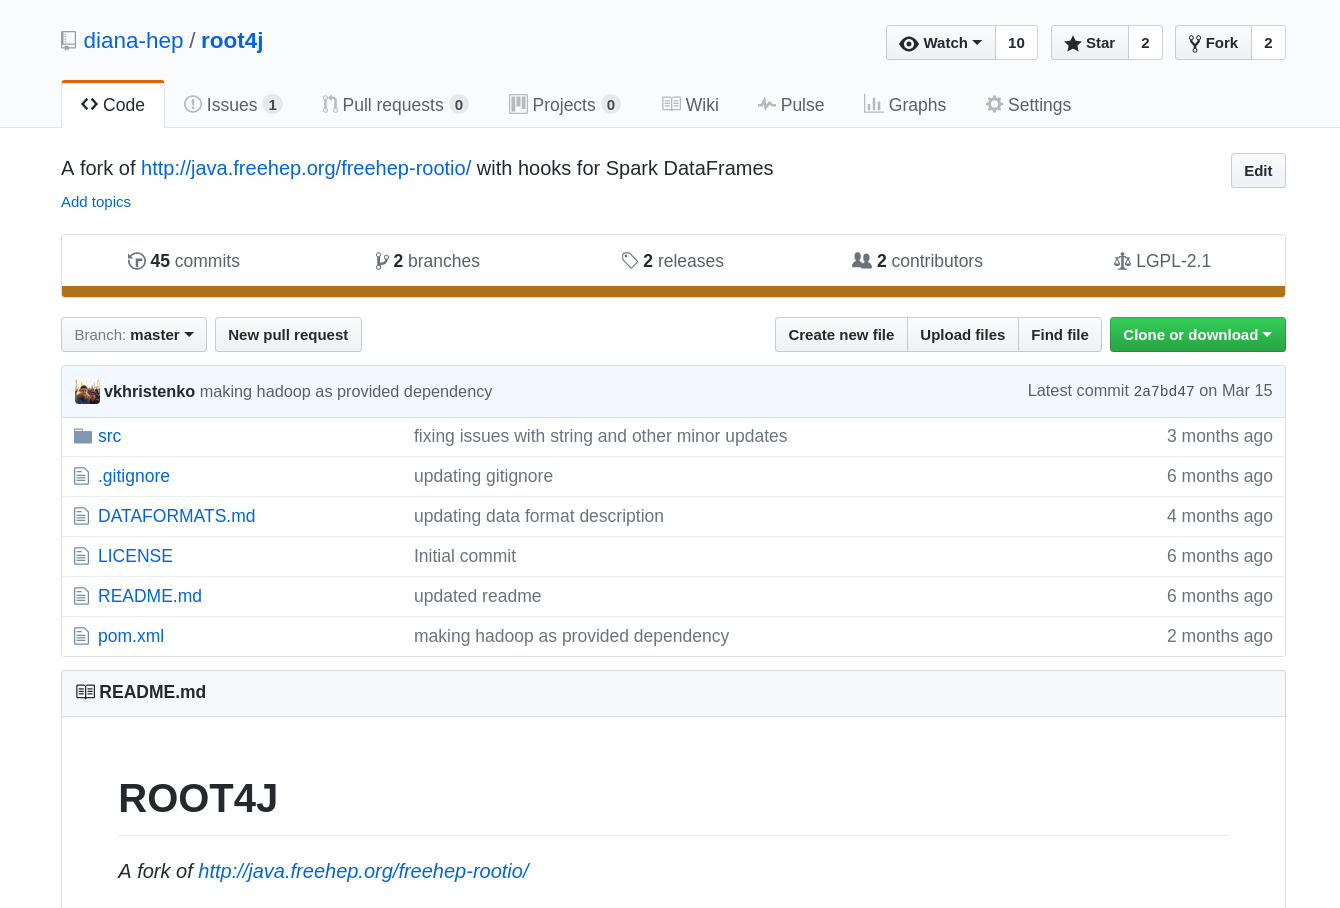
\includegraphics[width=\linewidth]{root4j.png}}}
\vspace{6 cm}
\end{columns}
\end{frame}

\begin{frame}[fragile]{Example session (\only<1>{native Spark, which is Scala}\only<2>{PySpark in Python})}
\vspace{0.35 cm}
\begin{center}
\begin{minipage}{0.9\linewidth}
Launch Spark with packages from Maven Central.
\small
\begin{onlyenv}<1>
\begin{minted}{bash}
spark-shell --packages org.diana-hep:spark-root_2.11:x.y.z, \
                       org.diana-hep:histogrammar_2.11:1.0.4
\end{minted}
\end{onlyenv}
\begin{onlyenv}<2>
\begin{minted}{bash}
pyspark     --packages org.diana-hep:spark-root_2.11:x.y.z, \
                       org.diana-hep:histogrammar_2.11:1.0.4
\end{minted}
\end{onlyenv}

\normalsize
Read ROOT files like any other DataFrame input source.

\small
\begin{onlyenv}<1>
\begin{minted}{scala}
val df = spark.sqlContext.read.root(
                          "hdfs://path/to/files/*.root")
\end{minted}
\end{onlyenv}
\begin{onlyenv}<2>
\begin{minted}{python}
df = sqlContext.read.format("org.dianahep.sparkroot") \
                    .load("hdfs://path/to/files/*.root")
\end{minted}
\end{onlyenv}

\vspace{-0.5 cm}
\small
\begin{verbatim}
df.printSchema()
root
 |-- met: float (nullable = false)
 |-- muons: array (nullable = false)
 |    |-- element: struct (containsNull = false)
 |    |    |-- pt: float (nullable = false)
 |    |    |-- eta: float (nullable = false)
 |    |    |-- phi: float (nullable = false)
 |-- jets: array (nullable = false)
\end{verbatim}
\end{minipage}
\end{center}
\end{frame}

\begin{frame}[fragile]{Example session (native Spark and PySpark)}
\vspace{0.35 cm}
\begin{center}
\begin{minipage}{0.9\linewidth}
\small
\begin{verbatim}
df.show()
+---------+--------------------+--------------------+
|      met|               muons|                jets|
+---------+--------------------+--------------------+
| 55.59374|[[28.07075,-1.331...|[[194.19714,-2.65...|
|39.440292|                  []|[[93.64958,-0.273...|
|2.1817229|[[5.523367,-0.375...|[[96.09923,0.7058...|
|  80.5822|[[48.910114,-0.17...|[[165.2686,0.2623...|
| 84.43806|                  []|[[51.87823,1.6442...|
| 84.63146|[[33.84279,-0.062...|[[137.74776,-0.45...|
| 393.8167|[[25.402626,-0.66...|[[481.8268,-1.115...|
|  75.0873|                  []|[[144.62373,-2.21...|
|2.6512942|[[6.851382,2.3145...|[[72.08256,-1.713...|
|36.753353|                  []|[[72.7172,-1.3265...|
+---------+--------------------+--------------------+
only showing top 10 rows
\end{verbatim}
\end{minipage}
\end{center}
\end{frame}

\begin{frame}[fragile]{Example session (\only<1>{Spark}\only<2>{PySpark})}
\vspace{0.1 cm}
\small
\begin{onlyenv}<1>
\begin{minted}{scala}
// Bring dollar-sign notation into scope.
import spark.sqlContext.implicits._


// Compute event weight with columns and constants.
df.select(($"lumi"*xsec/nGen) * $"LHE_weight"(309)).show()

// Pre-defined function (notation's a little weird).
val isGoodEvent = (
    ($"evtHasGoodVtx" === 1) &&
    ($"evtHasTrg" === 1)     &&
    ($"tkmet" >= 25.0)       &&
    ($"Mu_pt" >= 30.0)       &&
    ($"W_mt" >= 30.0))

// Use it.
println("%d events pass".format(
                    df.where(isGoodEvent).count()))
\end{minted}
\end{onlyenv}\begin{onlyenv}<2>
\begin{minted}{python}
# Python trick: make columns Python variables.
for name in df.schema.names:
    exec("{0} = df['{0}']".format(name))

# Look at a few event weights.
df.select((lumi*xsec/nGen) * LHE_weight[309]).show()

# Pre-defined function (notation's a little different).
isGoodEvent = (
    (evtHasGoodVtx == 1) &
    (evtHasTrg == 1)     &
    (tkmet >= 25.0)      &
    (Mu_pt >= 30.0)      &
    (W_mt >= 30.0))

# Use it.
print "{} events pass".format(
                  df.where(isGoodEvent).count())
\end{minted}
\end{onlyenv}
\end{frame}

\begin{frame}[fragile]{Example session (\only<1>{Spark}\only<2->{PySpark})}
\vspace{0.1 cm}
\small
\begin{onlyenv}<1>
\begin{minted}{scala}
// Use Histogrammar to make histograms.
import org.dianahep.histogrammar._
import org.dianahep.histogrammar.sparksql._
import org.dianahep.histogrammar.bokeh._

// Define histogram functions with SparkSQL Columns.
val h = df.Label(
         "muon pt" -> Bin(100, 0.0, 50.0, $"Mu_pt"),
         "W mt" -> Bin(100, 0.0, 120.0, $"W_mt"))

// Plot the histograms with Bokeh.
val bokehhist = h.get("muon pt").bokeh()
plot(bokehhist)
val bokehhist2 = h.get("W mt").bokeh()
plot(bokehhist2)
\end{minted}
\end{onlyenv}\begin{onlyenv}<2->
\begin{minted}{python}
# Use Histogrammar to make histograms.
from histogrammar import *
import histogrammar.sparksql
histogrammar.sparksql.addMethods(df)

# Define histogram functions with SparkSQL Columns.
h = df.Label(
      muon_pt = Bin(100, 0.0, 50.0, Mu_pt),
      W_mt = Bin(100, 0.0, 120.0, W_mt))

# Plot the histograms with PyROOT.
roothist = h.get("muon_pt").plot.root("muon pt")
roothist.Draw()
roothist2 = h.get("W_mt").plot.root("W mt")
roothist2.Draw()
\end{minted}
\end{onlyenv}

\vspace{-2.7 cm}
\begin{uncoverenv}<3>
\mbox{ } \hfill 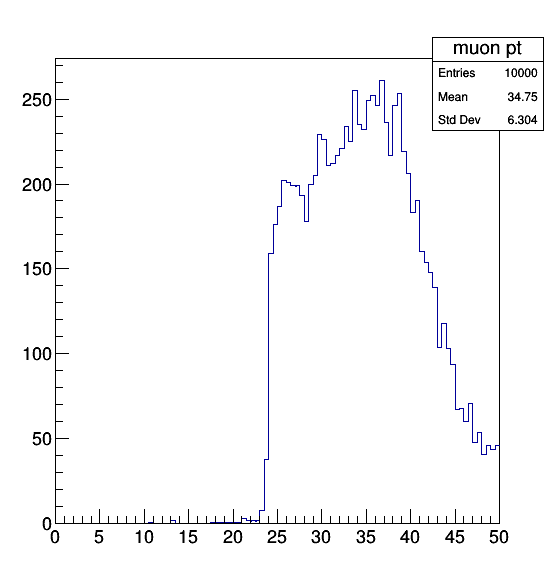
\includegraphics[width=3.8 cm]{muonpt.png}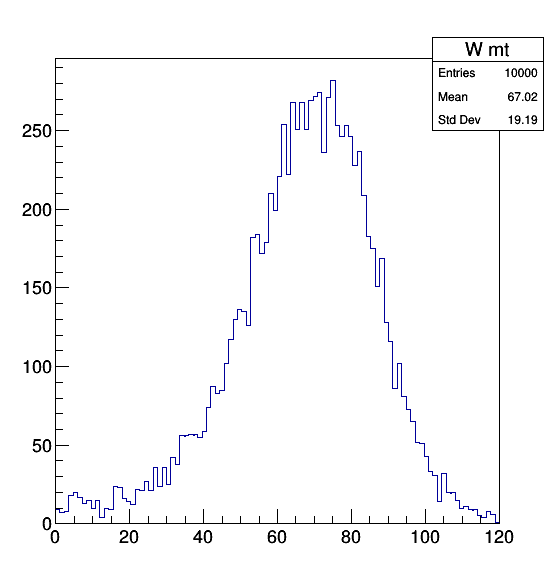
\includegraphics[width=3.8 cm]{wmt.png}
\end{uncoverenv}
\end{frame}

\begin{frame}{Speaking of plots\ldots}
\vspace{0.5 cm}
\begin{center}
\LARGE Spark and Big Data in general are weak in plotting.

\vspace{1 cm}
\uncover<2->{\Large They have fancy visualizations (d3), but lack convenient workaday routines for quick histograms, profiles, heatmaps, lego plots, etc.}

\vspace{1 cm}
\uncover<3->{\normalsize (Exception: Python and R have good interactive graphics for in-memory analytics.)}
\end{center}
\end{frame}

\begin{frame}[fragile]{Analysis in Spark is a chain of higher-order functions}
\vspace{1 cm}
\begin{columns}
\column{0.35\linewidth}
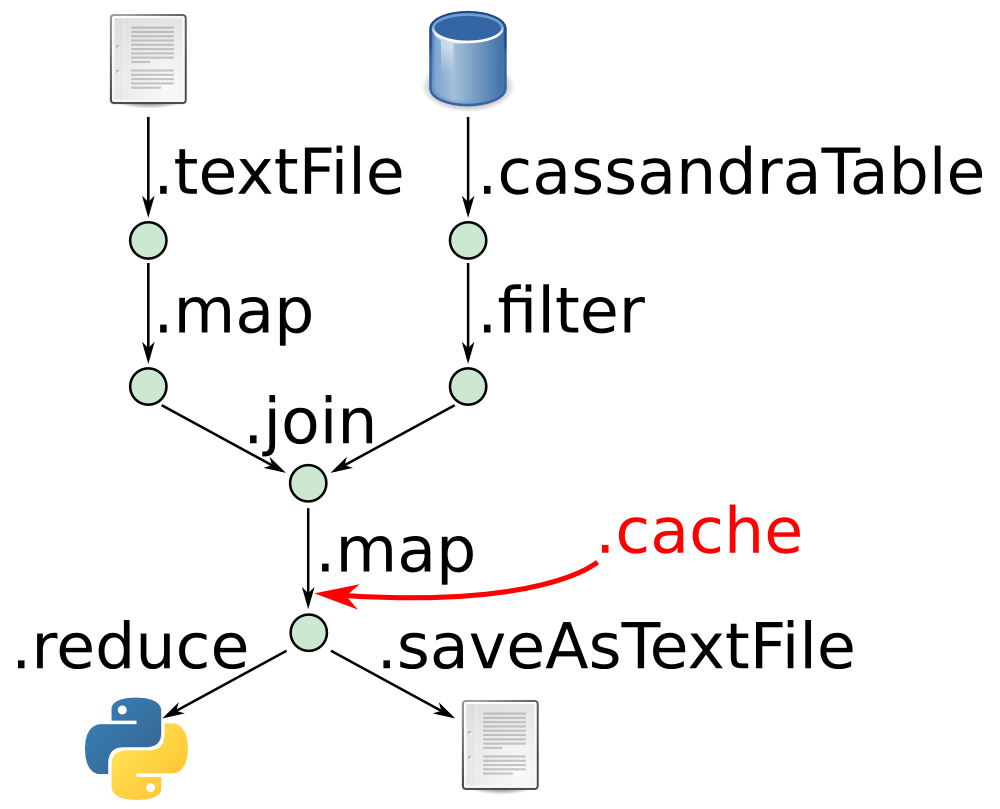
\includegraphics[width=\linewidth]{spark-dag.png}

\column{0.7\linewidth}
In Spark, you submit work by passing functions in a chain:

\small
\begin{minted}{scala}
one   = source1.textFile("some.txt")
               .map(x => x.upper())
two   = source2.cassandraTable
               .filter(x => x.field > 3)
three = one.join(two)
four  = three.map((x, y) => (y, x)).cache()
five  = four.reduce((x, y) => x + y)
six   = five.saveAsTextFile("other.txt")
\end{minted}
\end{columns}

\vspace{0.5 cm}
\begin{center}
\textcolor{darkblue}{\large Thus, the code doesn't depend on whether or not it's parallelized \\ (so it can be massively parallelized).}
\end{center}
\end{frame}

\begin{frame}[fragile]{ROOT histogram API is cumbersome in this setting}
\vspace{0.5 cm}
\begin{columns}
\column{0.5\linewidth}

\textcolor{darkblue}{ROOT (or any HBOOK-style) \mbox{histograms\hspace{-1 cm}}}
\small
\begin{minted}{python}
x = Histogram(100, -5.0, 5.0)

for event in events:
    x.fill(event.calcX())

x.plot()
\end{minted}

\column{0.52\linewidth}
\textcolor{darkblue}{Using them in Spark}
\small
\begin{minted}{python}
x = events.aggregate(
    Histogram(100, -5.0, 5.0),
    lambda h, event: (
        h.fill(event.calcX())),
    lambda h1, h2: (
        h1 + h2))

x.plot()
\end{minted}
\end{columns}
\end{frame}

\begin{frame}[fragile]{ROOT histogram API is cumbersome in this setting}
\vspace{0.5 cm}
\begin{columns}
\column{0.5\linewidth}

\textcolor{darkblue}{ROOT (or any HBOOK-style) \mbox{histograms\hspace{-1 cm}}}
\small
\begin{minted}{python}
x = Histogram(100, -5.0, 5.0)
y = Histogram(100, -5.0, 5.0)

for event in events:
    x.fill(event.calcX())
    y.fill(event.calcY())

x.plot()
y.plot()
\end{minted}

\column{0.52\linewidth}
\textcolor{darkblue}{Using them in Spark}
\small
\begin{minted}{python}
x, y = events.aggregate(
    (Histogram(100, -5.0, 5.0),
     Histogram(100, -5.0, 5.0)),
    lambda hs, event: (
        hs[0].fill(event.calcX()),
        hs[1].fill(event.calcY())),
    lambda hs1, hs2: (
        hs1[0] + hs2[0],
        hs1[1] + hs2[1]))

x.plot()
y.plot()
\end{minted}
\end{columns}
\end{frame}

\begin{frame}[fragile]{ROOT histogram API is cumbersome in this setting}
\vspace{0.5 cm}
\begin{columns}
\column{0.5\linewidth}

\textcolor{darkblue}{ROOT (or any HBOOK-style) \mbox{histograms\hspace{-1 cm}}}
\small
\begin{minted}{python}
x = Histogram(100, -5.0, 5.0)
y = Histogram(100, -5.0, 5.0)
z = Histogram(100, -5.0, 5.0)

for event in events:
    x.fill(event.calcX())
    y.fill(event.calcY())
    z.fill(event.calcZ())

x.plot()
y.plot()
z.plot()
\end{minted}

\column{0.52\linewidth}
\textcolor{darkblue}{Using them in Spark}
\small
\begin{minted}{python}
x, y, z = events.aggregate(
    (Histogram(100, -5.0, 5.0),
     Histogram(100, -5.0, 5.0),
     Histogram(100, -5.0, 5.0)),
    lambda hs, event: (
        hs[0].fill(event.calcX()),
        hs[1].fill(event.calcY()),
        hs[2].fill(event.calcZ())),
    lambda hs1, hs2: (
        hs1[0] + hs2[0],
        hs1[1] + hs2[1],
        hs1[2] + hs2[2]))

x.plot()
y.plot()
z.plot()
\end{minted}
\end{columns}
\end{frame}

\begin{frame}[fragile]{Solution: make the histograms functional, like the rest of Spark}
\vspace{0.5 cm}
Histogram constructor as a higher-order function:

\begin{center}
\fbox{\begin{minipage}{0.85\linewidth}
\vspace{0.25 cm}
\ttfamily\small\hspace{0.25 cm} h = Histogram(numBins, lowEdge, highEdge, \textbf{fillRule})
\vspace{0.25 cm}
\end{minipage}}
\end{center}

where {\ttfamily\small\textbf{fillRule}} is a function : {\it data} $\to$ $\mathbb{R}$ that determines which bin an element of {\it data} increments.

\begin{uncoverenv}<2->
\vspace{0.5 cm}
All domain-specific knowledge is in the constructor. The filling function may now be generic (and automated).

\begin{center}
\fbox{\begin{minipage}{0.85\linewidth}
\vspace{0.25 cm}
\ttfamily\small\hspace{0.25 cm} h.fill(datum) \hspace{1 cm}\textcolor{gray}{\textit{\# calls fillRule(datum) internally}}
\vspace{0.25 cm}
\end{minipage}}
\end{center}
\end{uncoverenv}
\end{frame}

\begin{frame}[fragile]{Familiar histogram types are now generated by combinators}
\vspace{0.5 cm}
\begin{columns}
\column{0.5\linewidth}
\small
\textcolor{darkblue}{\normalsize Histograms:}
\begin{minted}{python}
Bin(num, low, high, fillRule,
  Count())
\end{minted}

\vspace{0.25 cm}
\textcolor{darkblue}{\normalsize Two-dimensional histograms:}
\begin{minted}{python}
Bin(xnum, xlow, xhigh, xfill,
  Bin(ynum, ylow, yhigh, yfill,
    Count()))
\end{minted}

\vspace{0.25 cm}
\textcolor{darkblue}{\normalsize Profile plots:}
\begin{minted}{python}
Bin(xnum, xlow, xhigh, xfill,
  Deviate(yfill))
\end{minted}

{\normalsize where {\ttfamily\small Deviate} aggregates a mean and standard deviation.}

\column{0.5\linewidth}
\small
\textcolor{darkblue}{\normalsize Mix and match binning methods:}
\begin{minted}{python}
IrregularlyBin([-2.4, -2.1, -1.5,
    0.0, 1.5, 2.1, 2.4],
  filleta,
  Bin(314, -3.14, 3.14, fillphi,
    Count()))

SparselyBin(0.01, filleta,
  Bin(314, -3.14, 3.14, fillphi,
    Count()))

Categorize(fillByName,
  Bin(314, -3.14, 3.14, fillphi,
    Count()))
\end{minted}
\end{columns}
\end{frame}

\begin{frame}{It all got mathematical pretty fast\ldots}
\vspace{0.3 cm}
{\bf For transparent parallelization, combinators must}

\vspace{0.2 cm}
\begin{uncoverenv}<1>
\hspace{0.7 cm}{\bf be additive:}

\hspace{1.2 cm}independent of {\it whether} datasets are partitioned.

\vspace{-0.3 cm}
\[ \textcolor{darkblue}{\mbox{fill}(\mbox{data}_1 + \mbox{data}_2)} = \textcolor{darkblue}{\mbox{fill}(\mbox{data}_1) + \mbox{fill}(\mbox{data}_2)} \]
\end{uncoverenv}

\vspace{-0.5 cm}
\begin{uncoverenv}<1>
\hspace{0.7 cm}{\bf be homogeneous in the weights:}

\hspace{1.2 cm}fill weight 0.0 corresponds to no fill, 1.0 to simple fill, 2.0 to double-fill, \ldots

\vspace{-0.3 cm}
\[ \textcolor{darkblue}{\mbox{fill}(\mbox{data}, \mbox{weight})} = \textcolor{darkblue}{\mbox{fill}(\mbox{data}) \cdot \mbox{weight}} \]
\end{uncoverenv}

\begin{uncoverenv}<1>
\vspace{-4.0 cm}
\hfill $\left\}\mbox{\rotatebox{90}{\hspace{-0.3 cm}linear\hspace{1.3 cm}}\hspace{0.15 cm}}\right.$ \hspace{-0.9 cm}
\end{uncoverenv}

\vspace{0.3 cm}
\begin{uncoverenv}<1>
\hspace{0.7 cm}{\bf be associative:}

\hspace{1.2 cm}independent of {\it where} datasets get partitioned.

\vspace{-0.3 cm}
\[ \textcolor{darkblue}{(h_1 + h_2) + h_3} = \textcolor{darkblue}{h_1 + (h_2 + h_3)} \]
\end{uncoverenv}

\vspace{-0.7 cm}
\begin{uncoverenv}<1>
\hspace{0.7 cm}{\bf have an identity:}

\hspace{1.2 cm}for both the \textcolor{darkblue}{fill} and \textcolor{darkblue}{$+$} methods.

\vspace{-0.3 cm}
\[ \textcolor{darkblue}{h + 0} = \textcolor{darkblue}{h}\mbox{,\hspace{0.5 cm}} \textcolor{darkblue}{0 + h} = \textcolor{darkblue}{h}\mbox{,\hspace{0.5 cm}} \textcolor{darkblue}{\mbox{fill}(\mbox{data}, 0)} = \textcolor{darkblue}{0} \]
\end{uncoverenv}

\begin{uncoverenv}<1>
\vspace{-3.9 cm}
\hfill $\left\}\mbox{\rotatebox{90}{\hspace{-0.5 cm}monoid\hspace{1.1 cm}}\hspace{0.15 cm}}\right.$ \hspace{-0.9 cm}
\end{uncoverenv}
\end{frame}

\begin{frame}{}
\vspace{1.5 cm}
\begin{center}

\includegraphics[width=0.6\linewidth]{histogrammar-logo-paths.pdf}

\vspace{0.5 cm}
\Large \href{http://histogrammar.org}{\textcolor{blue}{\tt http://histogrammar.org}}
\end{center}

\vspace{1.5 cm}
\textcolor{mauve}{\LARGE (Get it?)}
\end{frame}

\begin{frame}{Other projects in development}
\vspace{0.5 cm}
\large
\begin{itemize}\setlength{\itemsep}{0.35 cm}
\item {\bf uproot}: fast reading of ROOT files into Numpy/Pandas/Apache Arrow.
\item {\bf Arrowed}: transpiling complex analysis functions to skip object materialization (like SQL term rewriting, but for objects in Arrow format).
\item Extending ROOT to use an object store database instead of seek points in a file (the ``petabyte ROOT file'' project).
\item Speeding up analysis cuts with database-style indexing.
\item {\bf Femtocode}: Domain Specific Language (DSL) for particle physics queries.
\end{itemize}

\vspace{0.2 cm}
\begin{uncoverenv}<2->
\textcolor{darkblue}{All of the above are parts of the following:}
\begin{itemize}\setlength{\itemsep}{0.5 cm}
\item To develop a centralized query service that is as responsive as a private skim:

to eliminate the need to copy data just to analyze it.
\end{itemize}
\end{uncoverenv}
\end{frame}

\begin{frame}{Conclusions}
\vspace{0.5 cm}
\begin{center}
\hspace{1 cm}\only<1>{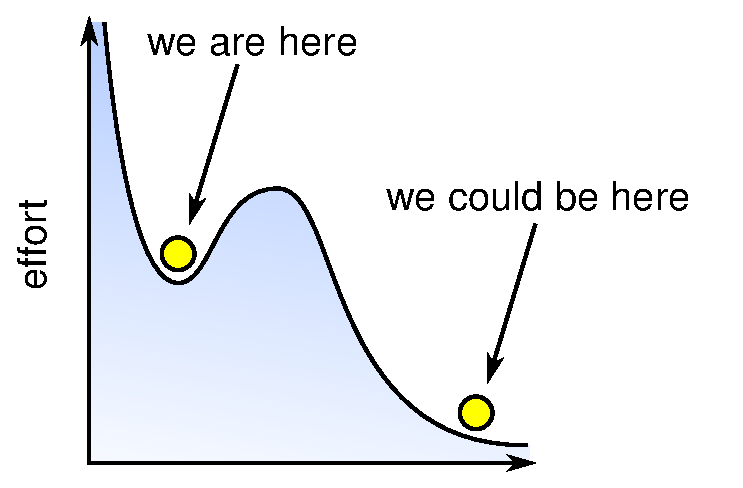
\includegraphics[width=0.65\linewidth]{effort0.pdf}}\only<2>{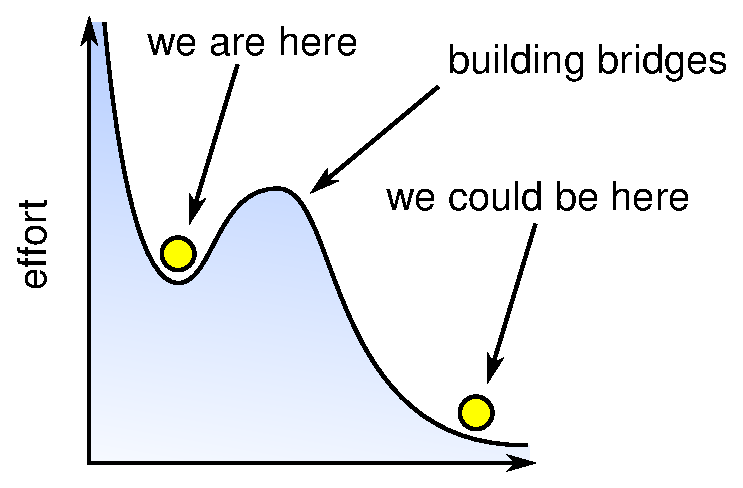
\includegraphics[width=0.65\linewidth]{effort.pdf}}
\end{center}
\end{frame}

\end{document}
